\documentclass{article}
\usepackage[utf8]{inputenc}
\usepackage[spanish]{babel}
\usepackage{listings}
\usepackage{graphicx}
\graphicspath{ {images/} }
\usepackage{cite}

\begin{document}

\begin{titlepage}
    \begin{center}
        \vspace*{1cm}
            
        \Huge
        \textbf{Desafío de objetos}
            
        \vspace{0.5cm}
        \LARGE
            
            
        \vspace{1.5cm}
            
        \textbf{Ferney Mejía Pérez}
            
        \vfill
            
        \vspace{0.8cm}
            
        \Large
        Departamento de Ingeniería Electrónica y Telecomunicaciones\\
        Universidad de Antioquia\\
        Caldas-Antioquia\\
        Marzo de 2021
            
    \end{center}
\end{titlepage}

\tableofcontents
\newpage
\section{Sección introductoria}\label{intro}
El objetivo principal de este trabajo es la realización y ejecución de una actividad propuesta por el docente guía del curso en proceso de Informática II, el cual está compuesto por un ejercicio inicial que hace énfasis en la descripción detallada de la traslación de un objeto ubicado en un punto A a un punto B. Además, tras realizar dicha actividad, se presenta la solución del problema mediante instrucciones a tres personas comunes con el fin de poner a prueba cuán óptimo y cuán comprensible es el resultado de dicho proceso.


\section{Sección de contenido} \label{contenido}
A continuación, se presentan cuatro secciones, en las cuales se describe el problema, la solución a este recurriendo a instrucciones, también, se expone el problema y la solución mediante imágenes, y por último, se adjunta un link al sitio web que almacena un vídeo contenedor del experimento con tres personas voluntarias dispuestas a poner a prueba la efectividad de dichas instrucciones.

\subsection{Problema}
Se tienen tres elementos que se presentan en la sección \ref{imagenes}, los cuales serán implementados para plantear el problema como tal.
Ahora bien, la condición inicial es la siguiente; se debe hacer uso de una superficie plana (mesa), en la cuál tras ubicar las tarjetas de igual tamaño y proporción por debajo de la hoja en blanco sobre dicha superficie, se debe proceder haciendo uso de sólo una mano, tratar de formar una pirámide como se indica en la figura \ref{fig:Piramide}.

\subsection{Instrucciones de solución}
1. Si la hoja en blanco está ubicada en posición vertical, girarla hasta que quede ubicada en posición horizontal.

2. Si la hoja está ubicada en posición horizontal omitir la instrucción 1.

3. Por condiciones naturales al posicionar de manera horizontal la hoja, se forma un rectángulo. Ahora bien, hacer un doblez en la parte superior del ancho del rectángulo hasta la mitad de la hoja. Repetir el proceso pero en la parte inferior del ancho del rectángulo. 

4. Por consiguiente, se presencia que la nueva forma de la hoja queda de manera similar a un plegable. Levantar la hoja desde cualquier parte tratando de mantener dicha forma, desplazarla unos cuantos centímetros a la derecha hasta presenciar las tarjetas y descargarla sobre la misma superficie plana inicial (mesa).

5. Si las tarjetas se encuentran desordenadas o regadas, sobreponer una ante la otra, levantarlas y desplazarlas unos centímetros a la izquierda sobre la superficie plana inicial(mesa) y descargarlas. 

6. Ahora, volver a sujetar la hoja en blanco manteniendo la forma del plegable y levantarla, esto para ubicarla en la posición inicial después de haber sido doblada sobre la superficie plana (mesa) de la cuál fue desplazada. Luego girar la hoja hacia arriba (90°) hasta quedar de forma vertical. 

7. Dirigirse hacia las tarjetas que deben estar sobrepuestas, sujetarlas con las yemas de los dedos manteniendo la sobreposición, luego, levantarlas de forma paralela a la superficie plana (mesa).

8. Después de levantar las tarjetas sobrepuestas, girar las tarjetas de manera horizontal hasta formar un rectángulo pequeño. Desplazar las tarjetas hasta quedar por encima de la hoja, y si se analiza la posición de las tarjetas y la hoja, se forma un eje coordenado (x,y).

9. Teniendo en cuenta esa imagen mental del eje coordenado (x,y), tratar de ubicar las tarjetas sobre el centro de la hoja (origen del eje), girar las tarjetas de manera que ambas estén de forma vertical y apoyarlas sobre la hoja.

10. Leer las instrucciones 11 y 12 antes de ejecutarlas.

11. Si la forma del plegable está cerrado, introducir ambas tarjetas por una de las aberturas (pestañas) que hacen parte del plegable, esto, hasta llegar al doblez que separa las paredes de dicho elemento, luego abrir la otra ala (pestaña) del plegable utilizando sólo una de las tarjetas hasta llegar al otro doblez y cerciorarse de que la hoja quede abierta. Después de haber ejecutado lo anterior, formar una pirámide con las tarjetas y saltar al paso 14.

12. Si la forma del plegable NO está cerrado, y la hoja en forma de plegable está abierto, ejecutar el paso 13 y 14 y omitir el 11.

13. Levantar el dedo meñique para mayor maniobrabilidad, luego deslizar levemente ambas tarjetas hacia los doblez de las hojas y sin permitir que se desplomen las tarjetas, formar una pirámide con las tarjetas.

14. Luego de formar la pirámide, liberar levemente el agarre de la mano a las tarjetas para evitar desplomar la figura.

\section{Inclusión de imágenes} \label{imagenes}
\begin{figure}[h]
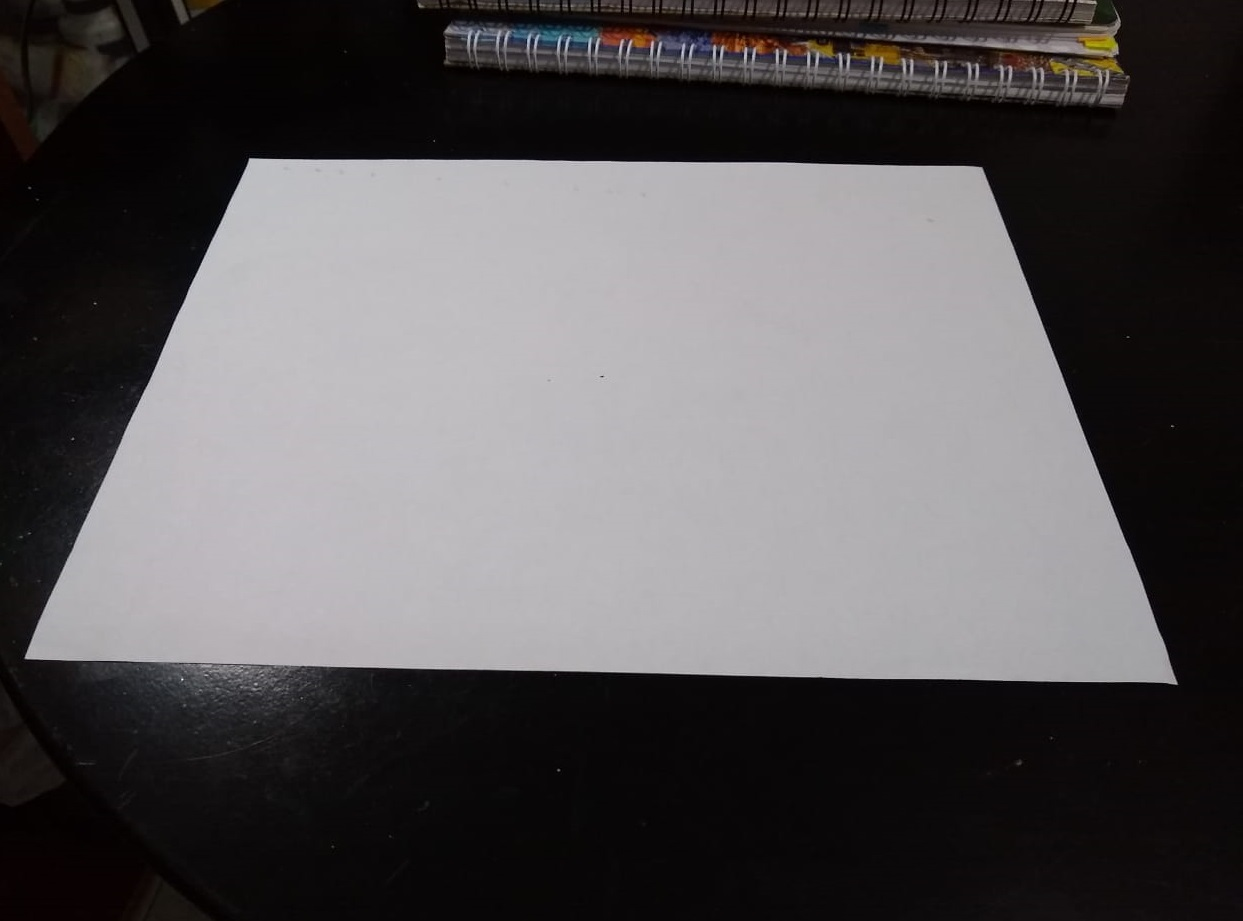
\includegraphics[width=4cm]{Hoja.jpeg}
\centering
\caption{Hoja en blanco}
\label{fig:Hoja}
\end{figure}
\begin{figure}[h]
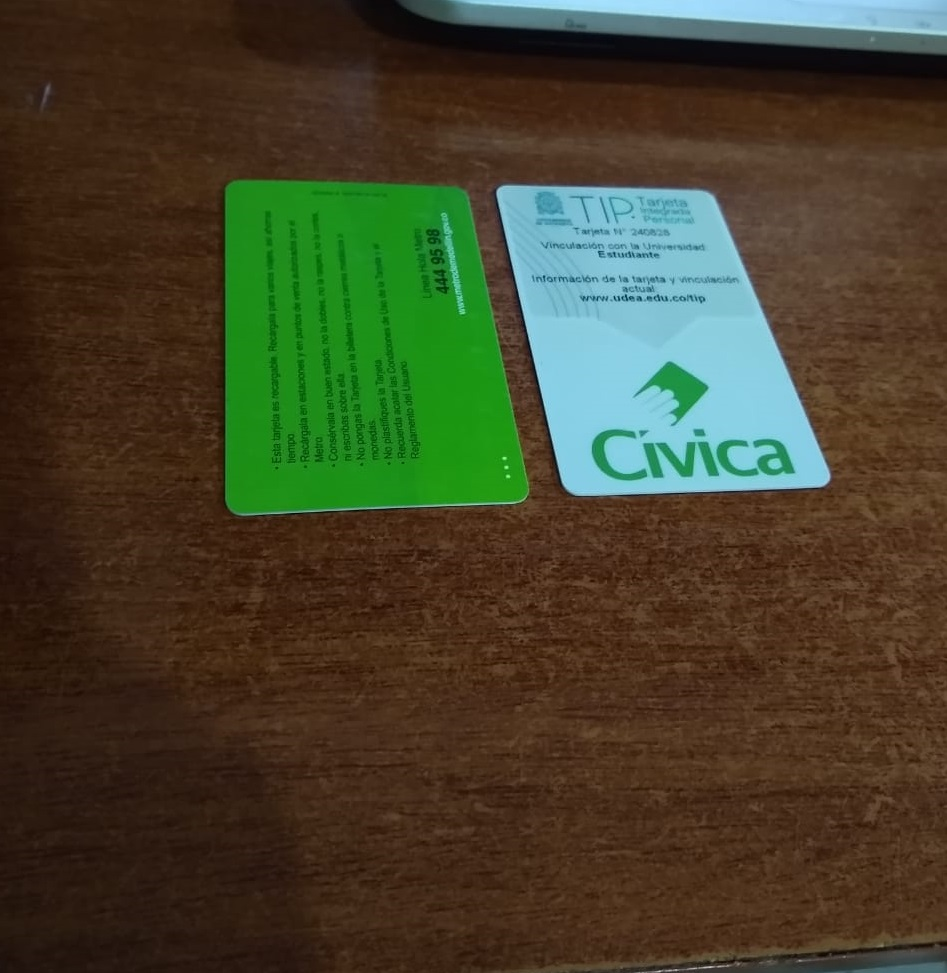
\includegraphics[width=4cm]{Tarjetas.jpeg}
\centering
\caption{Tarjetas de igual tamaño y proporción}
\label{fig:Tarjetas}
\end{figure}
\begin{figure}[h]
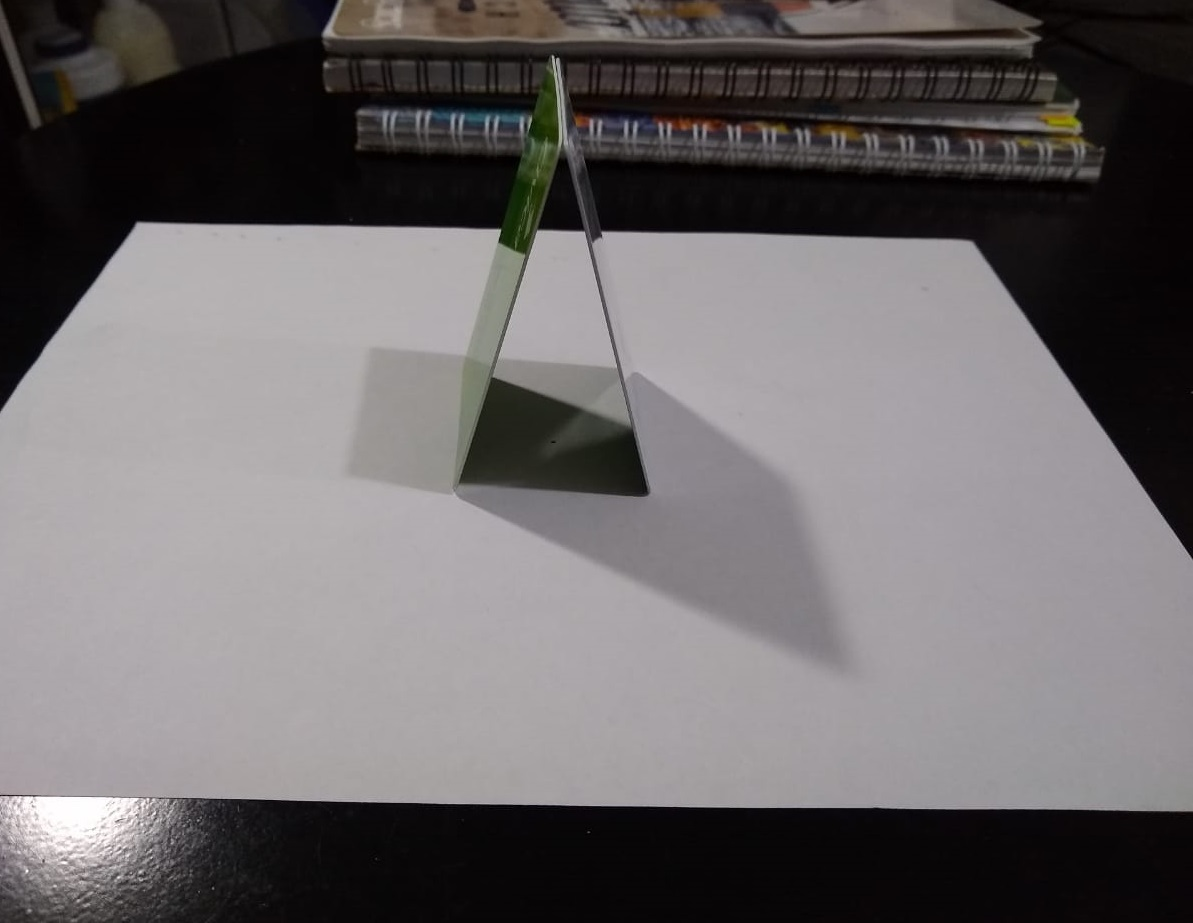
\includegraphics[width=5cm]{Piramide.jpeg}
\centering
\caption{Resultado esperado(pirámide)}
\label{fig:Piramide}
\end{figure}

\section{Link del experimento}
Haciendo uso de la plataforma de YouTube se añade el link del experimento realizado:

\newpage
\section{Reflexión}
Inicialmente el experimento falló con dos casos de prueba que realicé, por lo que me vi en la tarea de reformular parte de la solución que había exhibido, dado que habían instrucciones que generaban ambigüedad o en su defecto, faltaba información para completar la actividad.Luego, bajo la perspectiva de ser perfeccionista, insté en ejecutar varias veces las instrucciones que iba corrigiendo o añadiendo hasta llegar a un punto en el que una persona pudiera ejecutar sin mucha dificultad dichas instrucciones.

Ahora bien, es importante mencionar que este tipo de actividades nos ayudan a escatimar en detalles, desde lo más evidente hasta lo más complejo, pues, en el ámbito de la programación se vuelve necesario ser excesivamente minucioso para poder solventar las adversidades que se presentan cada vez que se desarrolla un proyecto y además, de que nos abre el pensamiento a un mundo de posibilidades que pueden existir al momento de tomar una decisión, también a enseñarnos a ver desde otras perspectivas y no pensar que la solución a un problema es única, es decir, cuando se programa nuestras mentes se enfocan en un punto y a veces, no tenemos en cuenta o ignoramos vertientes que pueden ser muy importantes, por lo que creemos que la soluciones que damos se vuelven infalibles y ahí es donde se comete errores. Así que, para finalizar considero que es muy importante como programador no sesgase a la idea de creer que todas las cosas hechas de primera vez puedan ser concluyentes, no, considero que una buena programación es un conjunto de pruebas y errores que nos ayudan a datar información sobre el cómo pensamos y el cómo ejecutamos las acciones sin premeditar, teniendo en cuenta unas palabras que si las analizamos bien sirven para este campo, y como decía Platón: "Pensar antes de actuar", en este campo, "Pensar antes de programar", para no perder tiempo más adelante.

\newpage
\section{Referencias}
\bibliographystyle{IEEEtran}
\bibliography{references}
\cite{calistenia}


\end{document}
